\documentclass[twocolumn,dvipdfmx]{jarticle}

\usepackage{jsaiac}
\usepackage{mymacros}
\usepackage{cite}
\usepackage{tabularx}
\newcolumntype{C}{>{\centering\arraybackslash}X}
\newcolumntype{R}{>{\raggedright\arraybackslash}X}
\newcolumntype{L}{>{\raggedleft\arraybackslash}X}

% 追加
\usepackage{adjustbox}
\usepackage{enumitem}
\usepackage{tcolorbox}
\usepackage{amsmath}
\usepackage{listings}
\usepackage{graphicx}
\usepackage{booktabs}

\definecolor{lightblue}{RGB}{242,242,254}
\lstset{
  backgroundcolor=\color{lightblue},
  frame=single,
  basicstyle=\ttfamily\footnotesize,
  breaklines=true,
  breakindent=0pt,
  breakautoindent=false
}

%%
\title{
\jtitle{友人関係ネットワークの6ヶ月間変化分析}
}

\affiliate{}

\author{
\jname{学籍番号: 82518829 氏名: 戸倉~健登}
}

\begin{document}
\setlength{\abovedisplayskip}{3pt}

\maketitle

\begin{abstract}
本レポートでは，ある集団における友人関係ネットワークの6ヶ月間の変化を分析した．
Cytoscapeを用いてネットワーク可視化と各種中心性指標の算出を行い，
ネットワーク構造の変化，中心人物の特定，性別・グループ間の関係パターンを考察した．
分析の結果，6ヶ月間でエッジ数が約46\%増加し，連結成分数が6から2に減少するなど
ネットワーク全体の結束性が高まったこと，
特定の女性ノードが媒介中心性を高め橋渡し役として機能していることが明らかになった．
\end{abstract}

\section{序論}

社会ネットワーク分析は，人々の関係性を定量的に理解するための重要な手法である．
本レポートでは，ある集団における友人関係ネットワークを対象に，
6ヶ月間でどのような構造変化が生じたかを分析する．

分析にはネットワーク可視化・分析ツールであるCytoscapeを使用し，
入次数中心性，媒介中心性，近接中心性などの指標を算出した．
また，性別やグループといった属性に基づくネットワークパターンの可視化も行った．

\section{データ概要}

\subsection{ネットワークの基本情報}

分析対象のネットワークは，6ヶ月前（Before）と6ヶ月後（After）の2時点で取得された
友人関係データである．各ノードは個人を表し，エッジは友人関係を示す有向グラフである．

表\ref{tab:network_overview}に両時点のネットワーク基本統計を示す．

\begin{table}[htbp]
\centering
\caption{ネットワーク基本統計}
\label{tab:network_overview}
\begin{tabular}{lcc}
\toprule
指標 & Before & After \\
\midrule
ノード数 & 37 & 41 \\
エッジ数 & 46 & 67 \\
平均隣接ノード数 & 2.16 & 2.83 \\
ネットワーク直径 & 4 & 5 \\
特性経路長 & 1.93 & 2.27 \\
クラスタ係数 & 0.091 & 0.177 \\
ネットワーク密度 & 0.035 & 0.041 \\
連結成分数 & 6 & 2 \\
\bottomrule
\end{tabular}
\end{table}

\subsection{ノード属性}

各ノードには以下の属性が付与されている：
\begin{itemize}
  \item \textbf{ID}: 個人識別番号
  \item \textbf{グループ}: 1〜4の4グループ
  \item \textbf{性別}: 男性(m)または女性(f)
\end{itemize}

ノードラベルは「ID-グループ(性別)」の形式で表現される．
例えば「23-1(f)」はID:23，グループ1，女性を意味する．

図\ref{fig:network_before}および図\ref{fig:network_after}に，
それぞれBefore・Afterのネットワーク全体像を示す．

\begin{figure}[htbp]
\centering
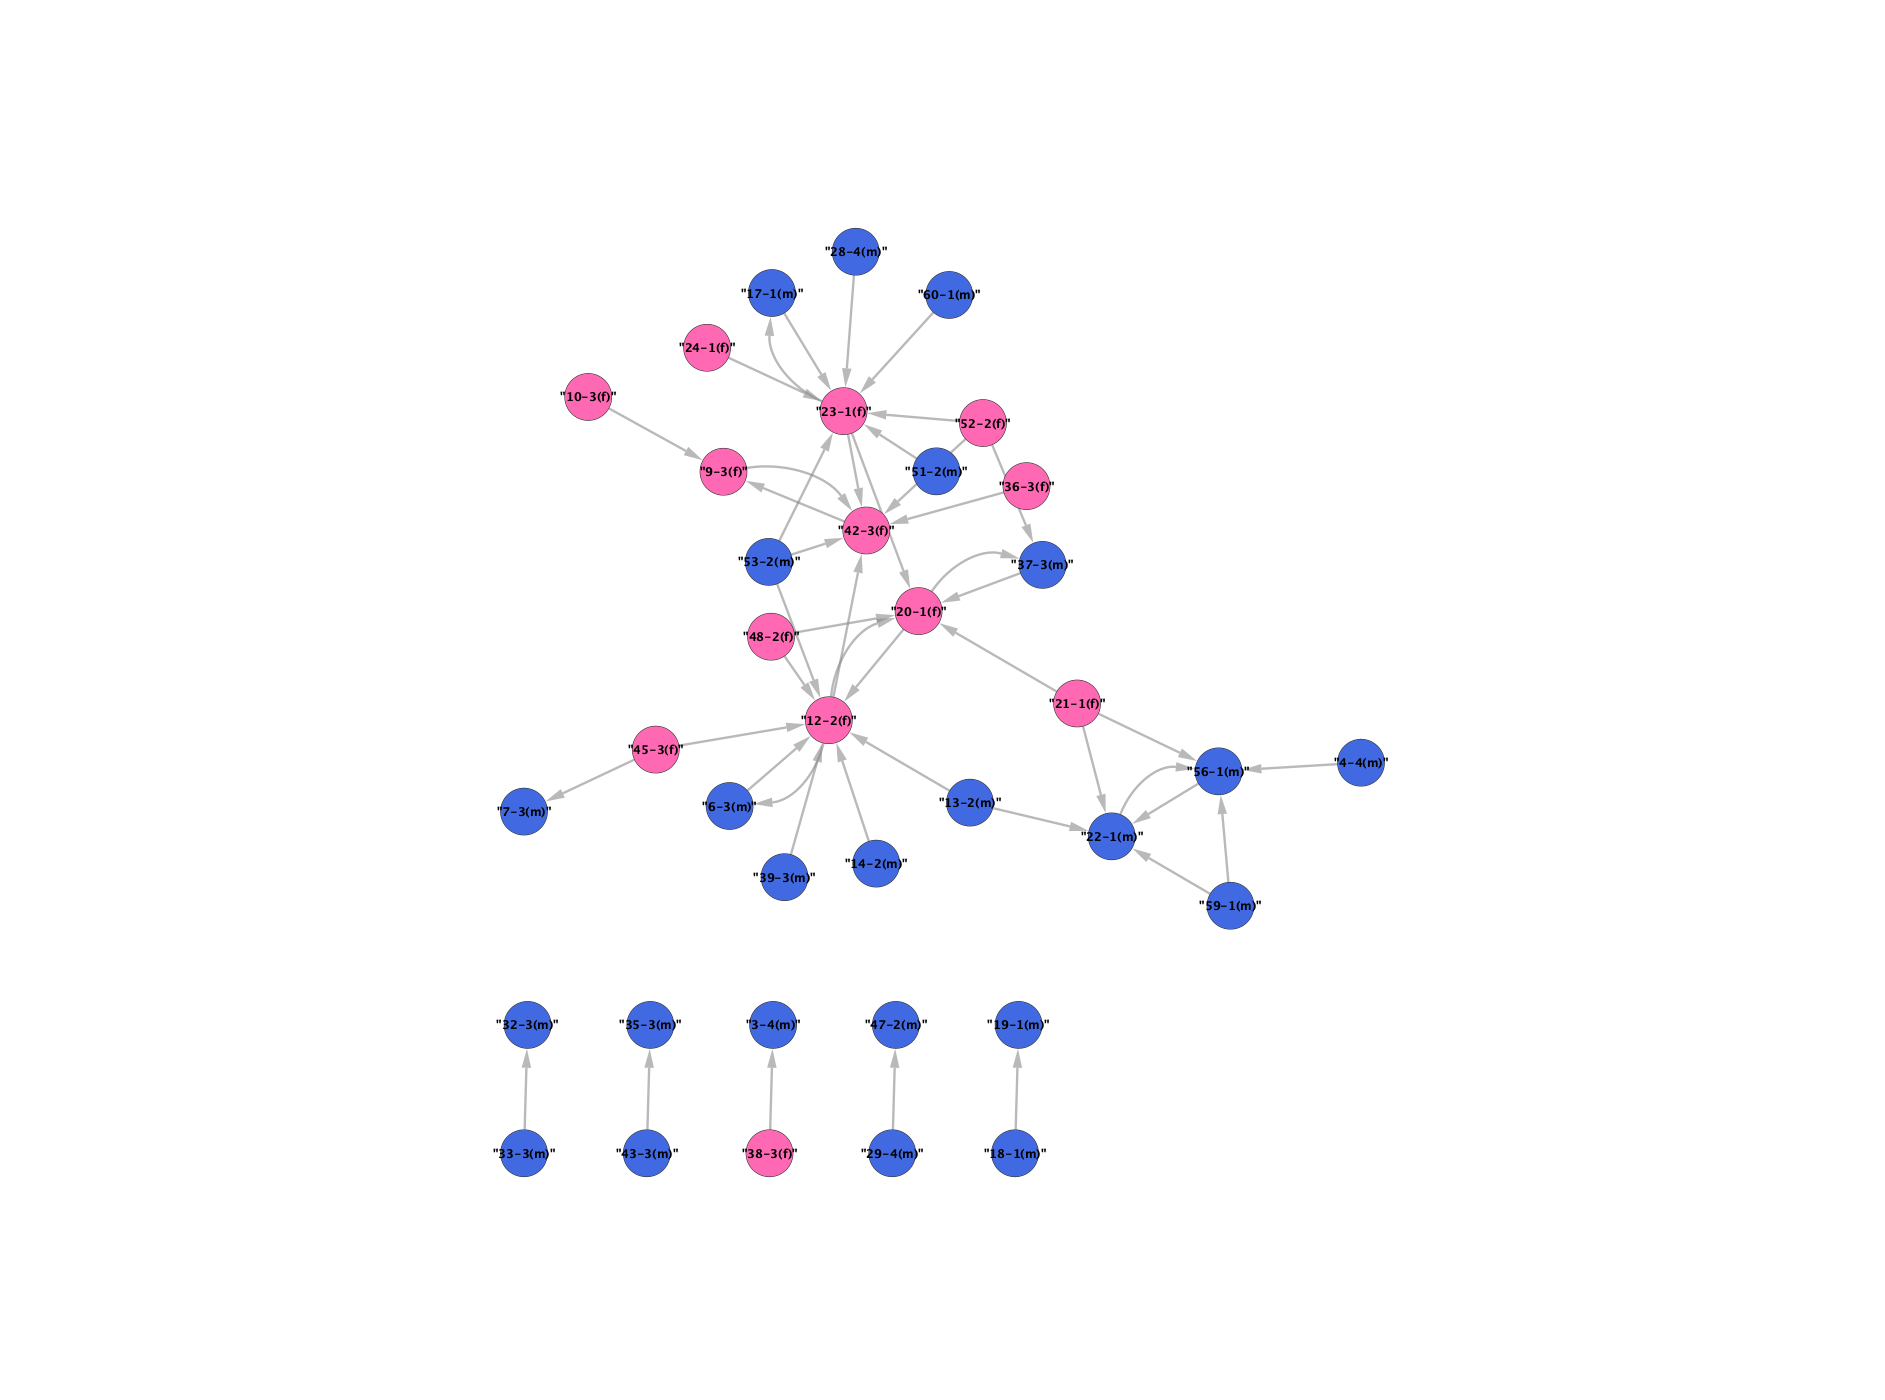
\includegraphics[width=0.95\linewidth]{fig/network_before.png}
\caption{Beforeネットワーク（6ヶ月前）．ノード色は性別を示す（ピンク：女性，青：男性）．矢印は友人関係の方向を表す．}
\label{fig:network_before}
\end{figure}

\begin{figure}[htbp]
\centering
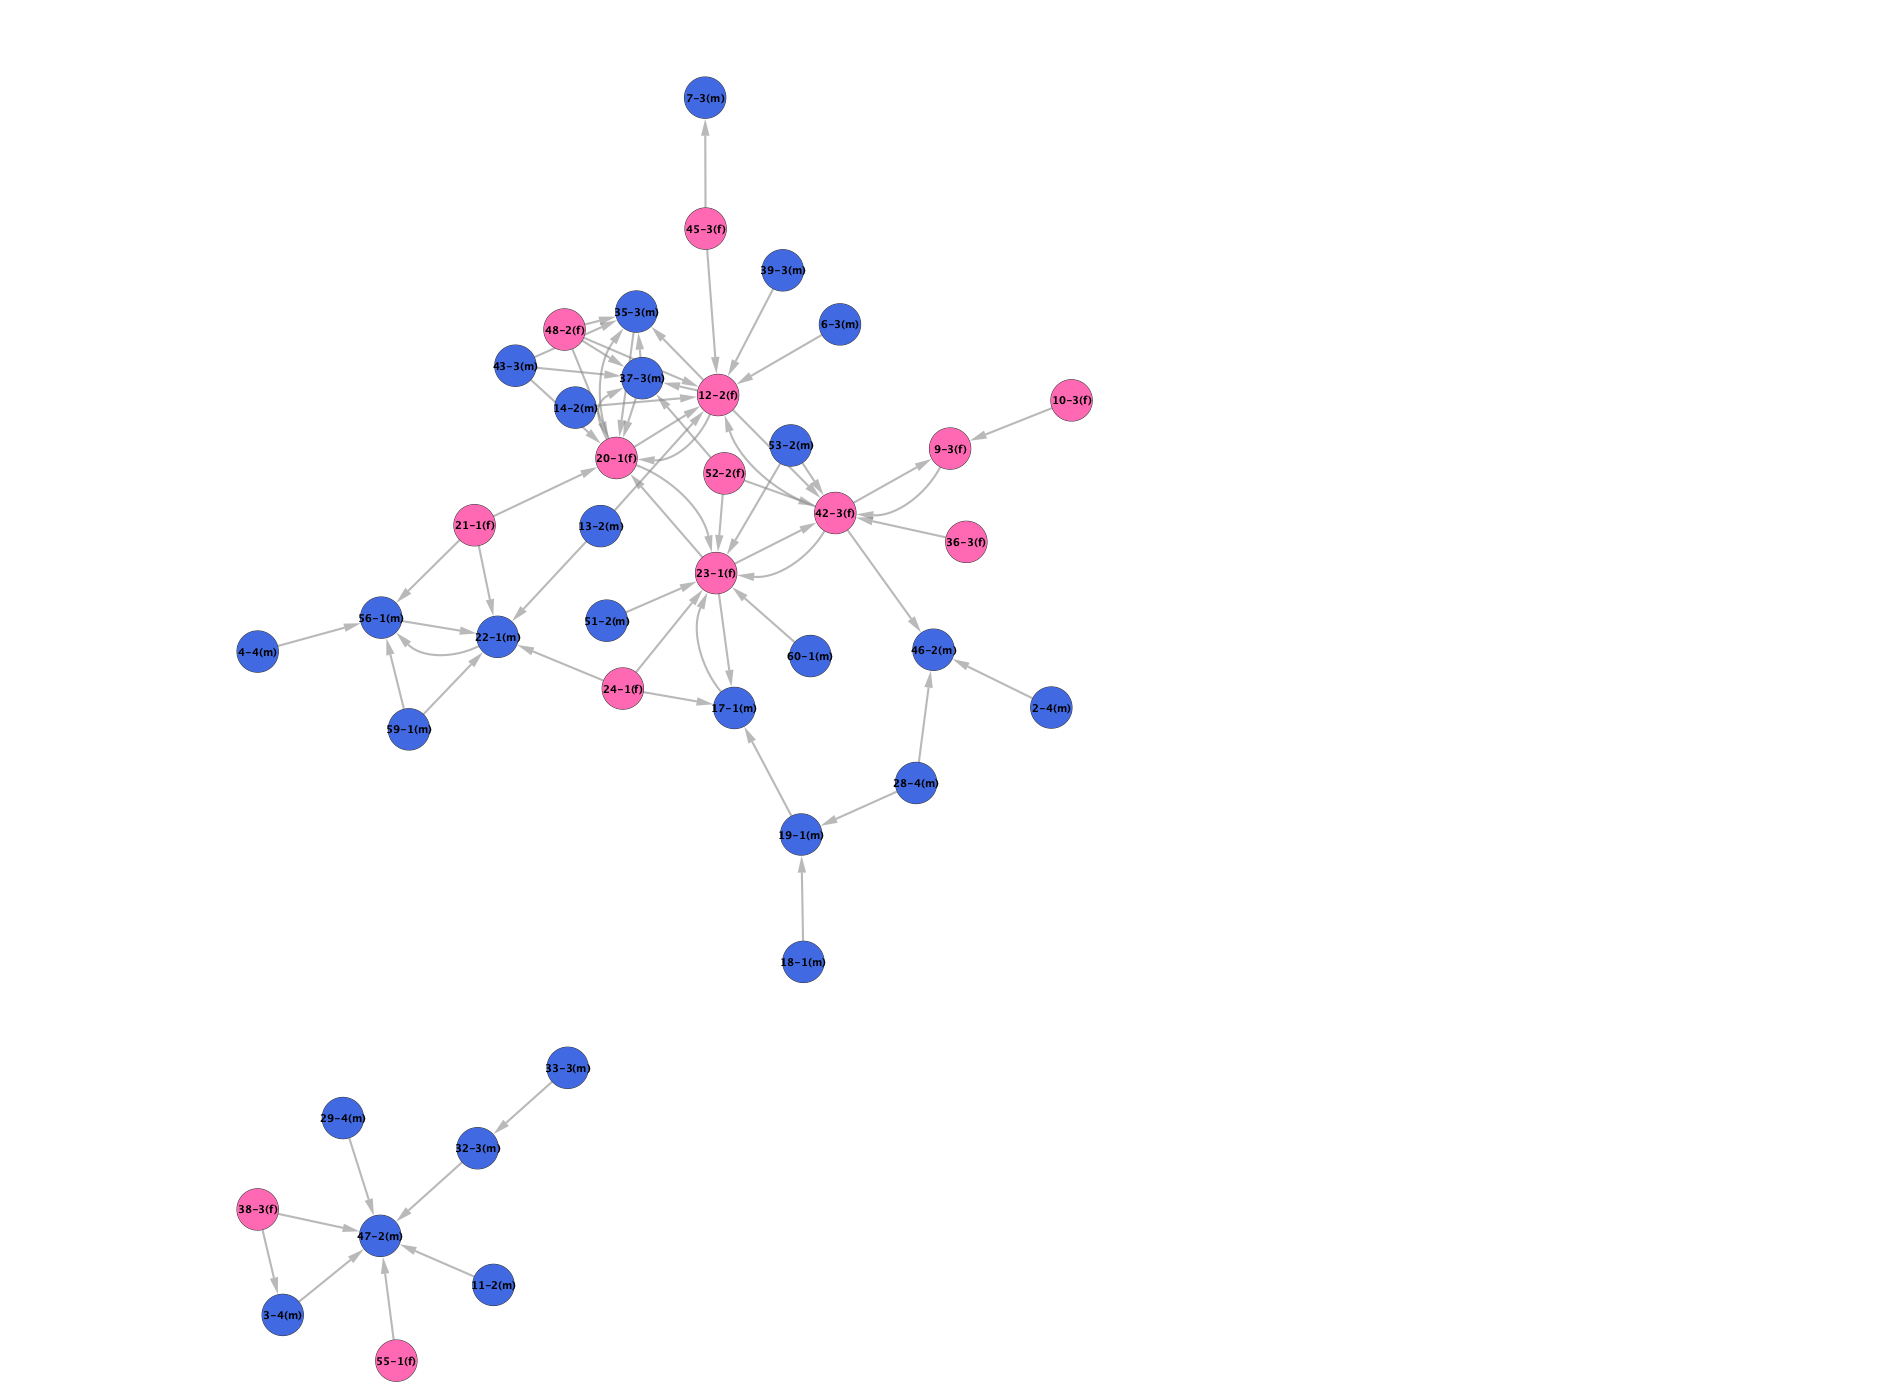
\includegraphics[width=0.95\linewidth]{fig/network_after.png}
\caption{Afterネットワーク（6ヶ月後）．ノード色は性別を示す（ピンク：女性，青：男性）．矢印は友人関係の方向を表す．}
\label{fig:network_after}
\end{figure}

\section{分析手法}

\subsection{使用ツール}

本分析ではCytoscape 3.10.4を使用した．
Cytoscapeはネットワーク可視化・分析のためのオープンソースソフトウェアであり，
生物学的ネットワークの解析を主目的として開発されたが，
社会ネットワーク分析にも広く利用されている．

\subsection{分析指標}

ネットワーク指標の算出には，Cytoscapeの「Tools → Analyze Network」機能を使用した．
この機能により，各ノードに対して次数，媒介中心性，近接中心性などの指標が自動的に計算され，
ノードテーブルに属性として追加される．
算出された指標値は，可視化スタイルのマッピングに使用できる．

以下の指標を算出し，ネットワーク構造を分析した：

\begin{itemize}
  \item \textbf{次数（Degree）}: ノード$v$に接続するエッジの総数．有向グラフでは入次数と出次数の合計となる：
  \[
    \text{Degree}(v) = \text{InDegree}(v) + \text{OutDegree}(v)
  \]
  友人の多さを示す．
  \item \textbf{入次数（InDegree）}: 他者から向けられたエッジ数．人気度を示す．
  \item \textbf{出次数（OutDegree）}: 自分から向けたエッジ数．積極性を示す．
  \item \textbf{媒介中心性（Betweenness Centrality）}: ノード$v$の媒介中心性$C_B(v)$は以下の式で計算される：
  \[
    C_B(v) = \sum_{s \neq v \neq t} \frac{\sigma_{st}(v)}{\sigma_{st}}
  \]
  ここで$\sigma_{st}$はノード$s$から$t$への最短経路の総数，$\sigma_{st}(v)$はそのうち$v$を経由する経路数である．この値が高いほど，異なるノード間を繋ぐ橋渡し役として重要であることを示す．
  \item \textbf{近接中心性（Closeness Centrality）}: ノード$v$から他の全ノードへの最短経路長の平均の逆数：
  \[
    C_C(v) = \frac{n-1}{\sum_{u \neq v} d(v, u)}
  \]
  ここで$d(v,u)$は$v$から$u$への最短経路長，$n$はノード数である．情報へのアクセス容易性を示す．
  \item \textbf{クラスタ係数（Clustering Coefficient）}: ノード$v$の隣接ノード間の接続密度：
  \[
    C(v) = \frac{2 \cdot e_v}{k_v(k_v - 1)}
  \]
  ここで$k_v$は$v$の隣接ノード数，$e_v$は隣接ノード間のエッジ数である．グループの結束度を示す．
\end{itemize}

\section{分析結果}

\subsection{入次数中心性分析}

図\ref{fig:degree_size}に，入次数（他者から友人として選ばれた数）に基づくノードサイズの可視化を示す．
ノードサイズが大きいほど多くの人から友人として選ばれていることを表す．

\begin{figure}[htbp]
\centering
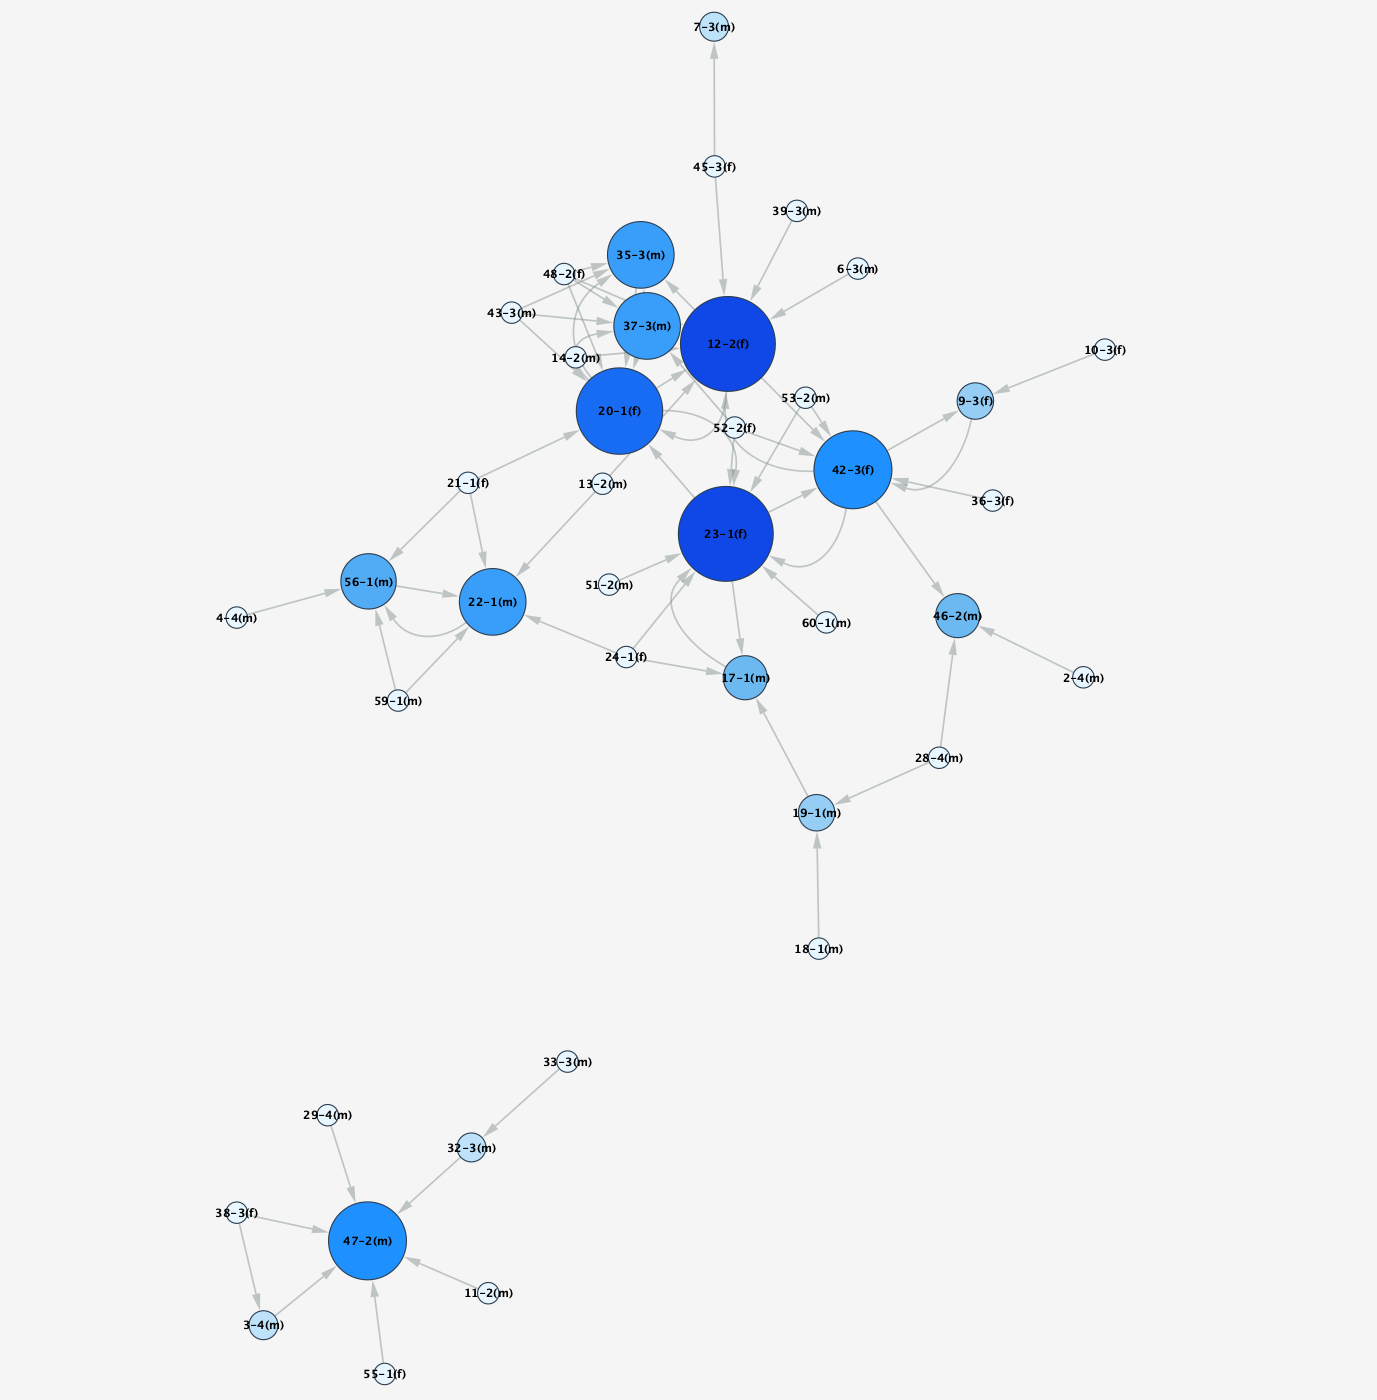
\includegraphics[width=0.95\linewidth]{fig/degree_size.png}
\caption{入次数中心性による可視化（Afterネットワーク）．ノードサイズと色は入次数に比例する（大きく濃いほど入次数が高い）．}
\label{fig:degree_size}
\end{figure}

Afterネットワークにおいて，特に入次数が高いノードとして
12-2(f)，20-1(f)，23-1(f)などが確認された．
これらのノードはネットワークにおいて人気が高く，ハブとして機能している．

\subsection{媒介中心性分析}

図\ref{fig:betweenness}に，媒介中心性に基づく可視化を示す．
可視化では，媒介中心性の値に応じてノードサイズと色を連続的にマッピングした．
具体的には，媒介中心性が0.0のノードは小さく薄い色（淡黄色），
0.5以上のノードは大きく濃い色（紫）となるグラデーションを適用した．
これにより，異なるグループを繋ぐ橋渡し役として重要なノードが視覚的に識別できる．

\begin{figure}[htbp]
\centering
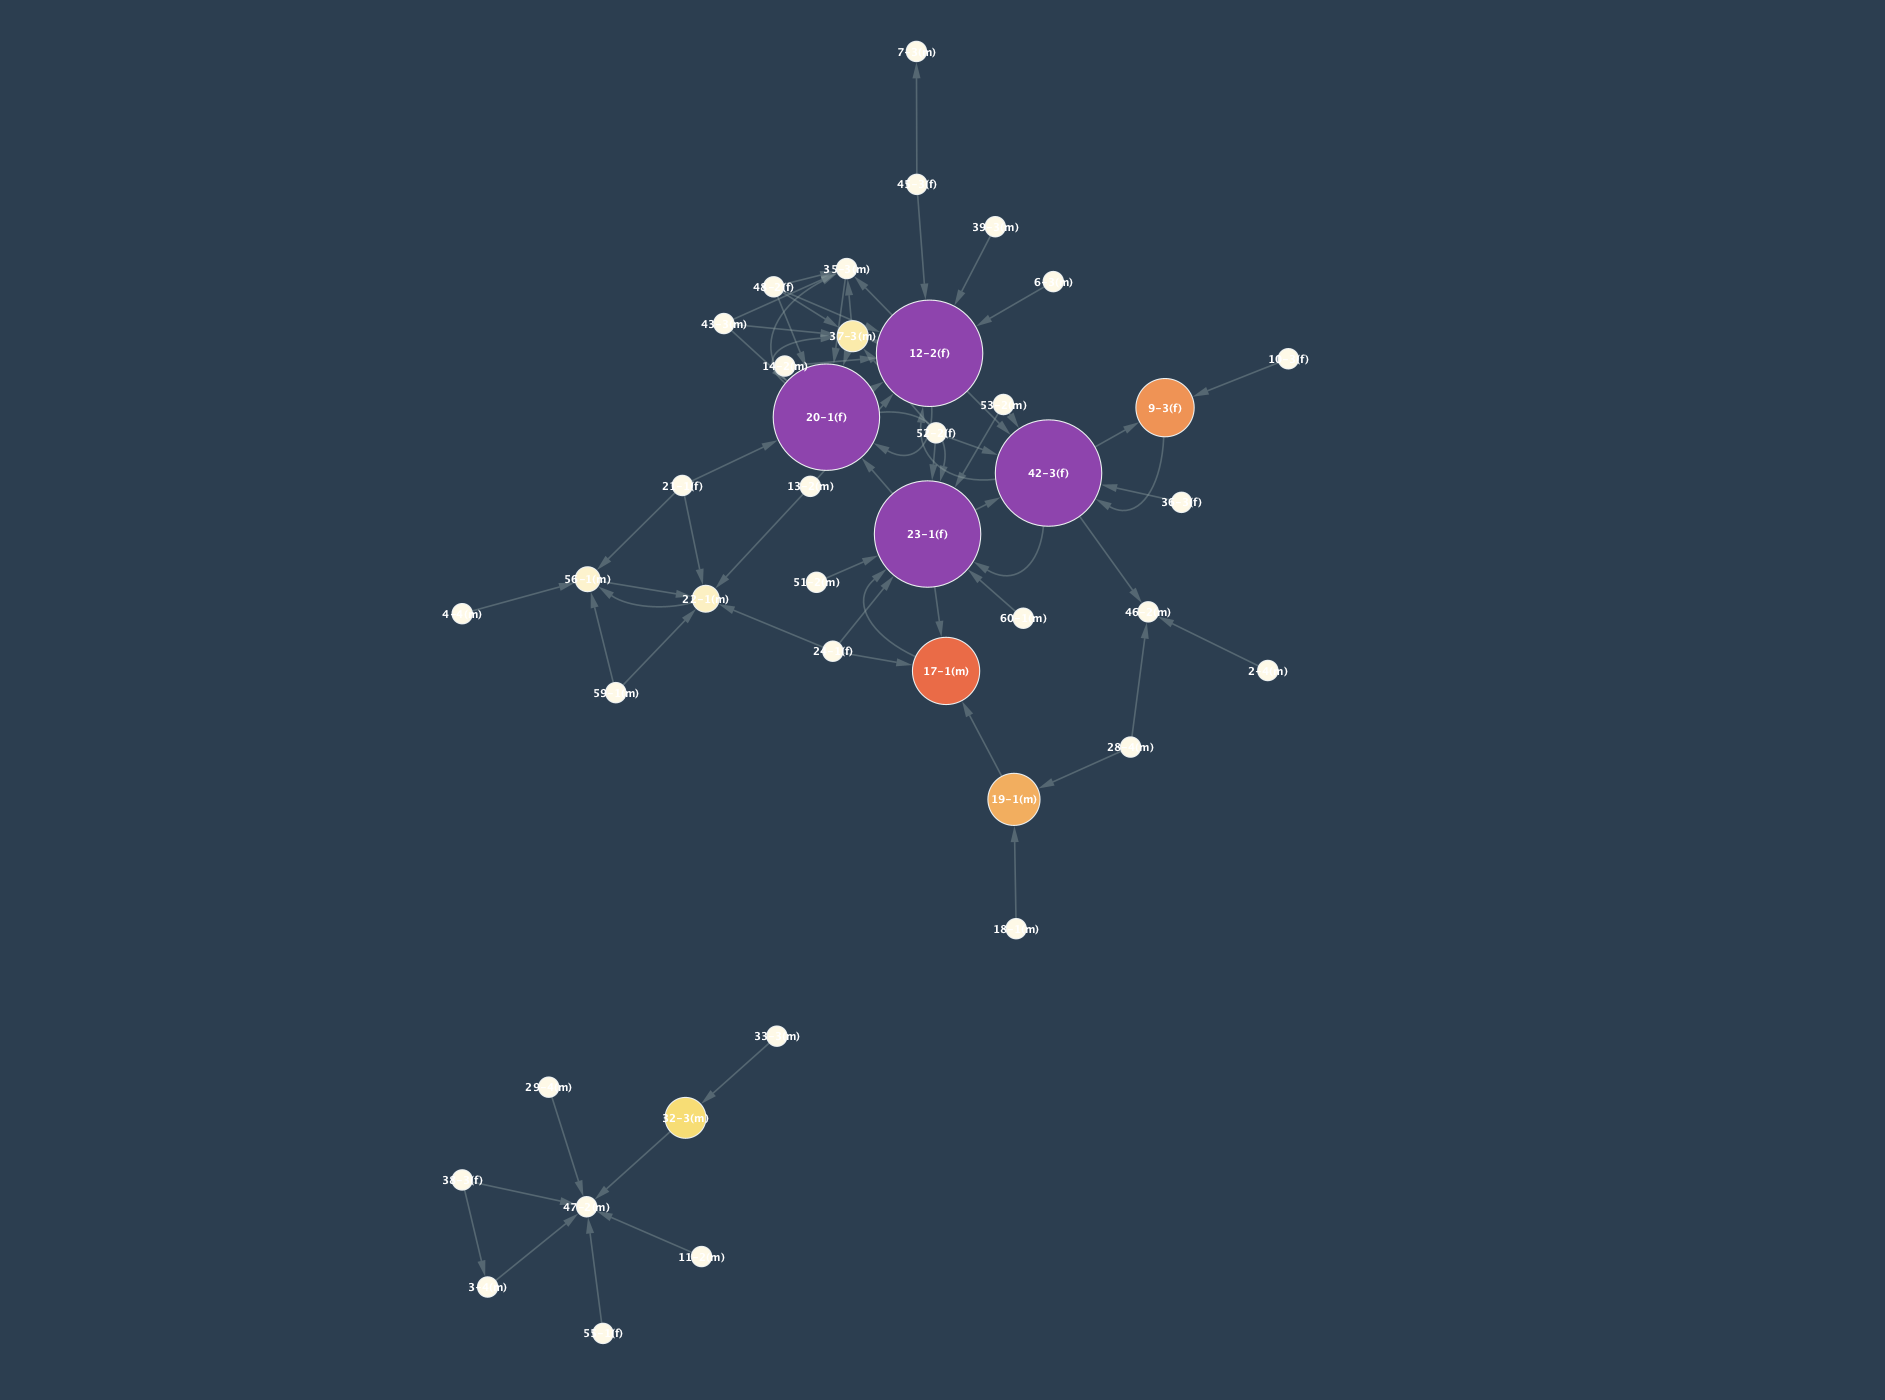
\includegraphics[width=0.95\linewidth]{fig/betweenness.png}
\caption{媒介中心性による可視化（Afterネットワーク）．ノードサイズと色は媒介中心性に比例する（大きく濃いほど橋渡し役として重要）．}
\label{fig:betweenness}
\end{figure}

媒介中心性が高いノードは，ネットワーク全体の情報伝達において重要な役割を果たす．
分析の結果，20-1(f)や23-1(f)が高い媒介中心性を示した．

\subsection{性別によるネットワークパターン}

図\ref{fig:network_before}および図\ref{fig:network_after}では，性別による色分け（ピンク：女性，青：男性）を適用している．

図\ref{fig:gender_edge}に，エッジの性別組み合わせによる色分けを示す．

\begin{figure}[htbp]
\centering
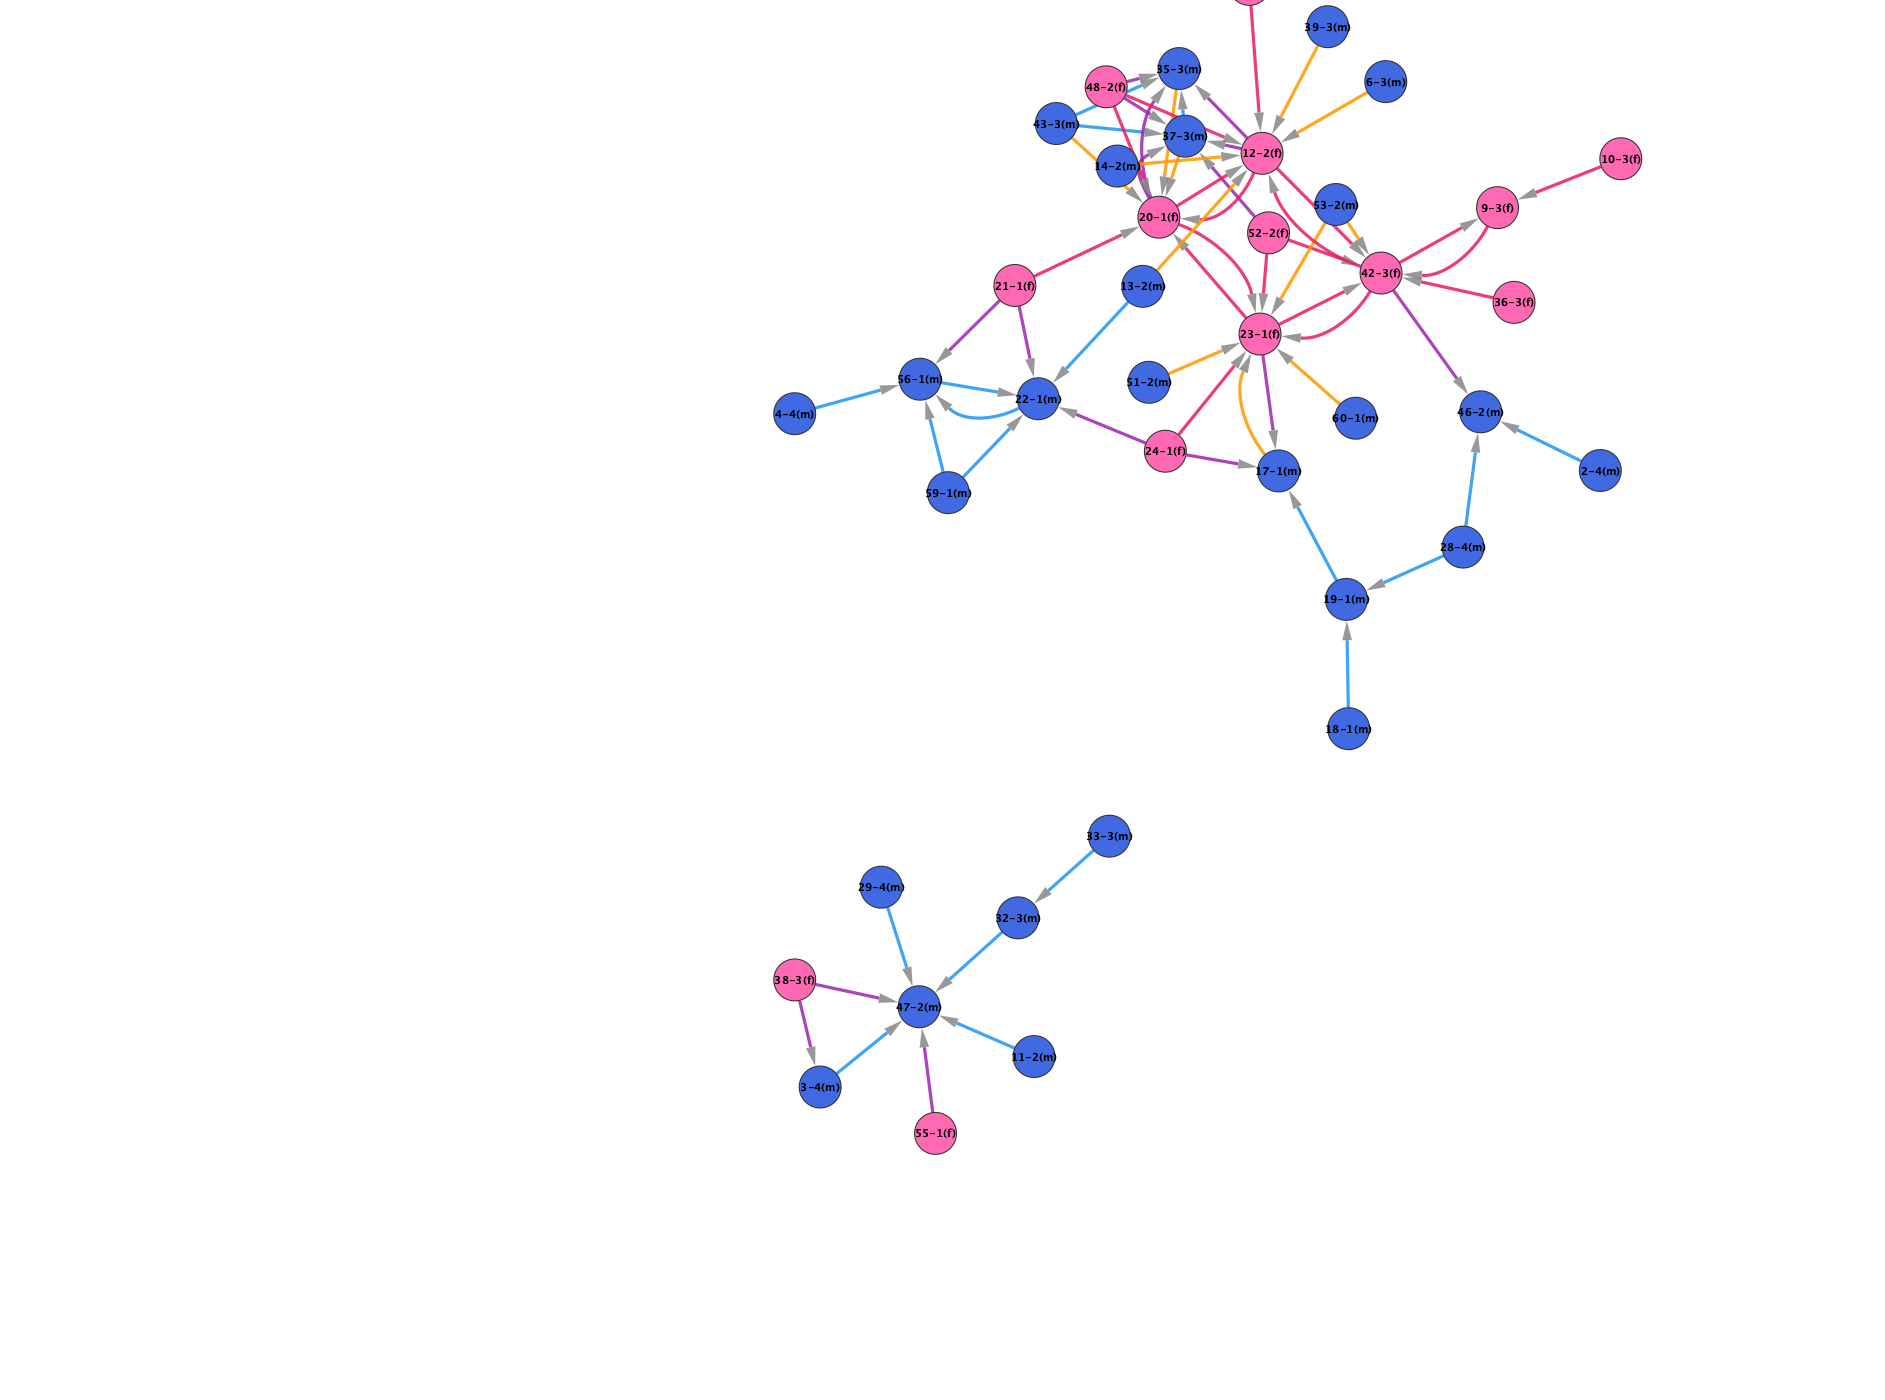
\includegraphics[width=0.95\linewidth]{fig/gender_edge.png}
\caption{エッジの性別組み合わせによる色分け（Afterネットワーク）．エッジ色：ピンク（女性→女性），紫（女性→男性），オレンジ（男性→女性），青（男性→男性）．ノード色：ピンク（女性），青（男性）．}
\label{fig:gender_edge}
\end{figure}

エッジの色分けは以下の通りである：
\begin{itemize}
  \item ピンク: 女性→女性
  \item 紫: 女性→男性
  \item オレンジ: 男性→女性
  \item 青: 男性→男性
\end{itemize}

\subsection{グループ間関係分析}

図\ref{fig:group_color}に，グループによる色分けを示す．
各ノードのグループ番号（ノードラベルの2番目の数字，例：「23-1(f)」のグループは1）に基づき，
離散的に色を割り当てた．

\begin{figure}[htbp]
\centering
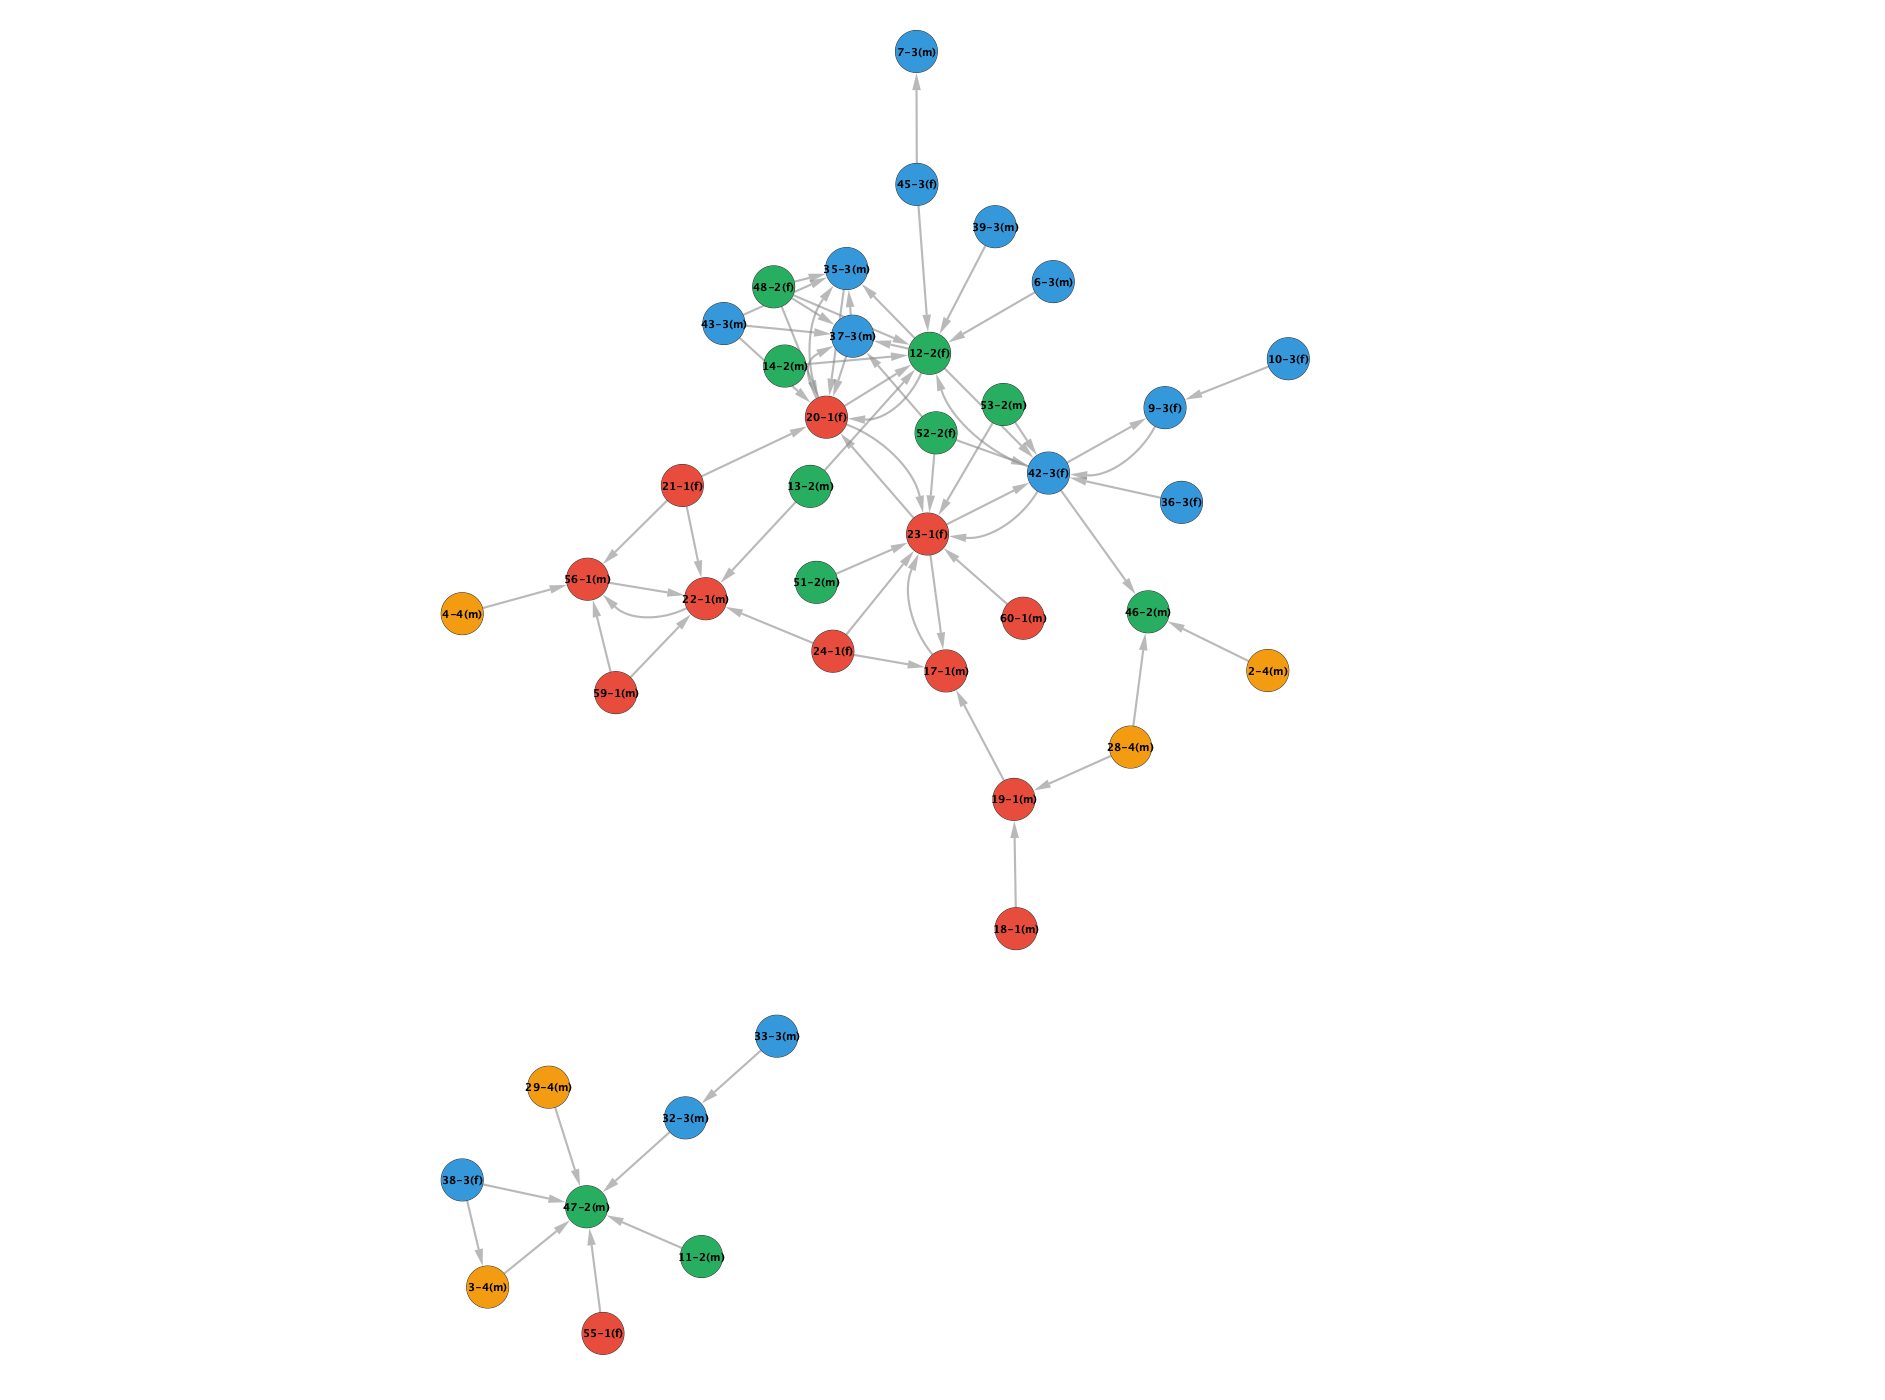
\includegraphics[width=0.95\linewidth]{fig/group_color.png}
\caption{グループによる色分け（Afterネットワーク）．ノード色はグループを示す（赤：グループ1，緑：グループ2，青：グループ3，オレンジ：グループ4）．}
\label{fig:group_color}
\end{figure}

グループ1（赤），グループ2（緑），グループ3（青），グループ4（オレンジ）で
ノードを色分けした結果，グループ間にも友人関係が形成されていることが確認できた．
特にグループ1と2の間，グループ2と3の間に多くのエッジが観察された．

\section{考察}

\subsection{6ヶ月間の構造変化}

6ヶ月間でノード数は37から41へ（+4名），エッジ数は46から67へ（+21本，約46\%増）と
ネットワークが拡大・緻密化した．
これは，既存メンバー間の新規関係形成と，新規メンバーの参加の両方が
寄与していることを示唆する．

\subsection{中心人物の役割}

入次数中心性と媒介中心性の分析から，以下の特徴が明らかになった：

\begin{itemize}
  \item 女性ノード（特に12-2(f)，20-1(f)，23-1(f)）が高い中心性を示した
  \item これらのノードはグループ間を繋ぐ橋渡し役としても機能している
  \item 男性ノードは比較的小規模なクラスタを形成する傾向が見られた
\end{itemize}

\subsection{性別・グループ間パターン}

エッジの性別組み合わせ分析から，以下のパターンが観察された：

\begin{itemize}
  \item 同性間のエッジ（f→f，m→m）が一定数存在
  \item 異性間のエッジも多く，特に女性が中心となる異性間ネットワークが形成されている
  \item グループ間のエッジも存在し，完全に分離されたコミュニティではない
\end{itemize}

\subsection{ネットワークの連結性}

連結成分分析の結果，Beforeネットワークでは6つの連結成分が存在したが，
Afterネットワークでは2つに減少した．
これは，6ヶ月間で孤立していたサブグループがメインのネットワークに統合されたことを示す．
クラスタ係数も0.091から0.177へと約2倍に増加しており，
ネットワーク全体の結束性が高まったことがわかる．

\section{結論}

本レポートでは，Cytoscapeを用いて友人関係ネットワークの6ヶ月間の変化を分析した．
主な知見は以下の通りである：

\begin{enumerate}
  \item ネットワークは6ヶ月間でエッジ数が約46\%増加し，より密な構造へと変化した
  \item 連結成分数が6から2に減少し，孤立グループの統合が進んだ
  \item 特定の女性ノード（12-2(f)，20-1(f)，23-1(f)）がハブおよび橋渡し役として機能
  \item クラスタ係数が約2倍に増加し，ネットワーク全体の結束性が高まった
\end{enumerate}

今後の課題として，時系列でのより詳細な変化追跡，
属性情報を用いた統計的検定，
および他の集団との比較分析が挙げられる．


\end{document}
